\subsubsection{Exercise}
\label{exo421}

Since $G_d(s) = \frac{10}{s+1}$, the cross-over frequency is $\omega_c = 10$ rad/s.

We have the following result:

$$\forall \omega < \omega_c, |Gd(j\omega)| >1$$

Control action is needed at least for $\omega \in [0,\omega_c]$.

Here, we will try to design $F_y$ in such a way that:
$$L(s) = F_y G \approx \frac{\omega_c}{s}$$

\paragraph{Unproper feedback}
Let:
$$F_y = G^{-1} \frac{\omega_c}{s} = \frac{200 s^3 + 4200 s^2 + 84000 s + 80000}{160000 s}$$

This controller has $3$ zero and $1$ pole.
Thus, it is not proper.
However -- using \texttt{Matlab} -- we can plot the step response of the system and the step response to a step perturbation (see Figure \ref{stepProper421}).

% \begin{figure}[h!t]
%     \centering
%     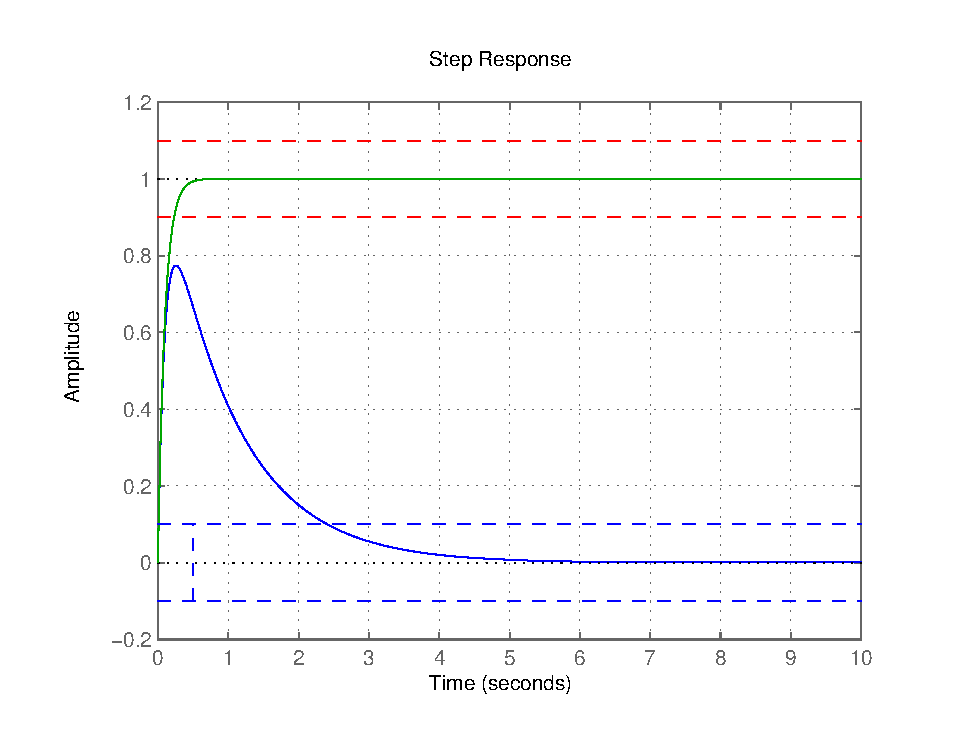
\includegraphics[width=\linewidth]{fig/stepNonProper421bis.eps}
%     \caption{Non-proper step response of the system}
%     \label{stepNonProper}
% \end{figure}
 
Figure \ref{stepProper421} shows that even if the performance are poor (With a step disturbance, $|y(t)| \leq 0.1$ for $t \geq t_d = 2.5$ s) we still have an attenuation of the perturbation and a step response of good quality (No overshoot and $t_r = 0.22$s).

\paragraph{Proper feedback}
Assuming that this controller is the one we want to implement, we need to design it in a proper way.
For now, it has $3$ zeros and $1$ pole.
Therefore it is needed to add two more poles.

Let:
$$F_y(s) = G^{-1}\frac{\omega_c}{s} \frac{\omega_1 \omega_2}{(s+\omega_1)(s+\omega_2)}$$

We need to choose $\omega_{1,2}$ in order to not change the system performance two much.

We use the following criteria:

\begin{shortitemize}
    \item $\omega_1 = \omega_2$
    \item $\omega_1$ and $\omega_2$ take action after $\omega_c$ 
\end{shortitemize}

Let's pick $\omega_1 = \omega_2 = \omega_0 = 100\omega_c$.
Figure \ref{bodeProper421} shows the bode diagram of $L(s) = F_y(s) G(s)$ (we can see that $\forall \omega < \omega_c, |L_{proper}|_{dB} \approx |L_{unproper}|_{dB}$).
Figure \ref{stepProper421} shows that the step response to a perturbation with $L_{proper}$ is the same than with $L_{unproper}$.

\begin{figure}[h!t]
    \includegraphics[width=\columnwidth]{fig/bodeProper421.eps}
    \caption{Bode diagram of $L(s)$ with the proper \& unproper $F_y$} 
    \label{bodeProper421}
\end{figure}

\begin{figure}[h!t]
    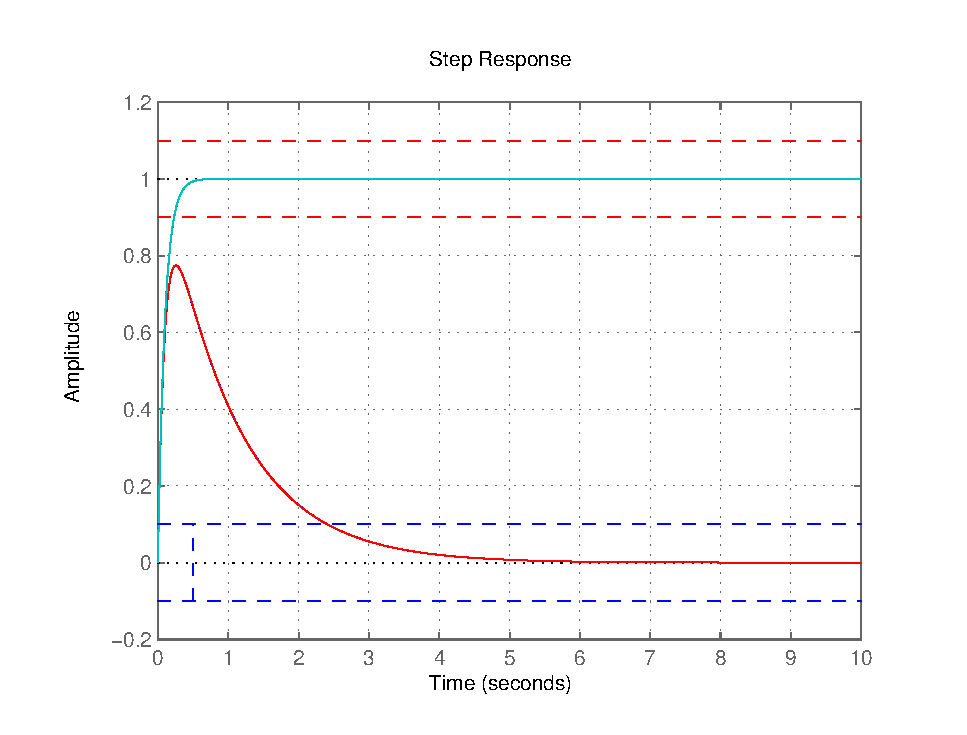
\includegraphics[width=\columnwidth]{fig/stepProper421bis.eps}
    \caption{Step response of the system with the proper \& unproper $F_y$ \\ Both responses are merged} 
    \label{stepProper421}
\end{figure}

